\beginsong{Das Gegenlied}[wuw={Claumisch (Michael Schmidt), VCP Bad Hersfeld "Mückenstürmer"}, pfii={180}, pfiii={95}, index={Ich singe hier kein Lied, dass ihr schon kennt}]

\markboth{\songtitle}{\songtitle}

\beginverse
\endverse
\centering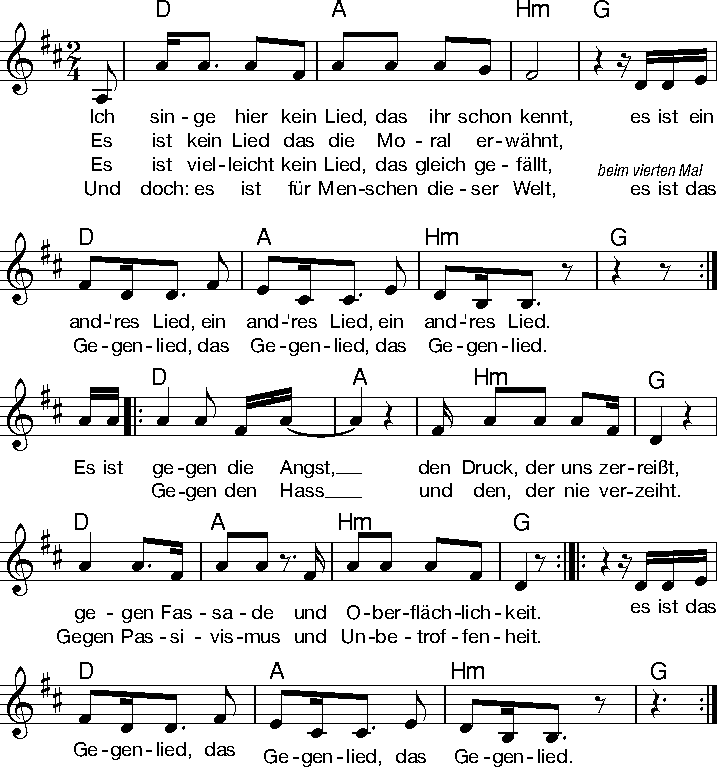
\includegraphics[width=1\textwidth]{Noten/Lied014.pdf}

\beginverse
Es \[D]ist kein Lied, das \[A]irgendwas be\[Hm]weist. \[G]
Es ist ein \[D]and'res Lied, ein \[A]and'res Lied, ein \[Hm]and'res Lied. \[G]
Es \[D]ist auch kein's, das \[A]tiefe Gräben \[Hm]reißt. \[G]
Es ist ein \[D]and'res Lied, ein \[A]and'res Lied, ein \[Hm]and'res Lied. \[G]
Kein \[D]Damokles\[A]schwert, das \[Hm]über uns \[G]schwebt.
Es ist ein \[D]and'res Lied, ein \[A]and'res Lied, ein \[Hm]and'res Lied. \[G]
Wenn \[D]jeder nur ein \[A]bisschen danach \[Hm]lebt, \[G]
es ist ein \[D]Lebenslied, ein \[A]Lebenslied, ein \[Hm]Lebenslied! \[G]
\endverse
 
\beginchorus
Es ist \[D]gegen die \[A]Angst, den \[Hm]Druck der uns zer\[G]reißt,
\[D]gegen Fas\[A]sade und \[Hm]Oberflächlich\[G]keit,
\[D]gegen den \[A]Hass und \[Hm]den der nie ver\[G]zeiht,
\[D]gegen Passi\[A]vismus und \[Hm]Unbetroffen\[G]heit.
\lrep Es ist das \[D]Gegenlied, das \[A]Gegenlied, das \[Hm]Gegenlied. \[G] \rrep \newline

Es \[D]ist für den Mut zum \[A]Widerstand und \[Hm]für die Offen\[G]heit,
\[D]für Akti\[A]vismus und \[Hm]Unbequemlich\[G]keit,
für \[D]Liebe und für \[A]Hoffnung, \[Hm]Gefühle jeder\[G]zeit,
\[D]für Kontro\[A]versen \[Hm]und für Ehrlich\[G]keit.
\lrep Es ist ein \[D]Lebenslied, ein \[A]Lebenslied, ein \[Hm]Lebenslied!\[G]\rrep - \[D]
\endchorus

\endsong

\beginscripture{}
% nix g'fund'n
\endscripture

\begin{intersong}

\end{intersong}